\section{Реализация программного комплекса калибровки результатов рекомендательных системы}
\subsection{Выбор технологий и инструментов для реализации}
Для программной реализации методов калибровки рекомендательных систем были выбраны следующие инструменты:
\begin{itemize} 
    \item Python3 -- скриптовый динамический язык программирования, 
    выбран для реализации методов и использования готовых библиотек.
    \item SurPrise \cite{sur} -- фреймворк для языка программирования Python
    с готовой реализацией нескольких методов рекомендательных систем.
    \item SciPy \cite{Scipy} -- это бесплатная библиотека Python с открытым исходным кодом, используемая для научных вычислений и технических вычислений.
    \item Implicit \cite{imp} -- библиотека с реализованной коллаборативной фильтрацией для неизвестных данных.
  \end{itemize}

\subsection{Алгоритм рекомендательной системы}

В качестве алгоритма рекомендаций было выбрано Байесовское 
персонализированное ранжирование \cite{bib8}. 
Основная задача персонализированного ранжирования состоит 
в том, чтобы предоставить пользователю ранжированный список 
элементов.

Пусть ${U}$-множество всех пользователей,а ${I}$-множество всех 
элементов. Ниже на рисунке \ref{BPR1} показано, как обрабатываются неявные 
данные в случае общих рекомендателей элементов.
\begin{figure}[ht]
    \begin{center}
    \scalebox{0.35}{
       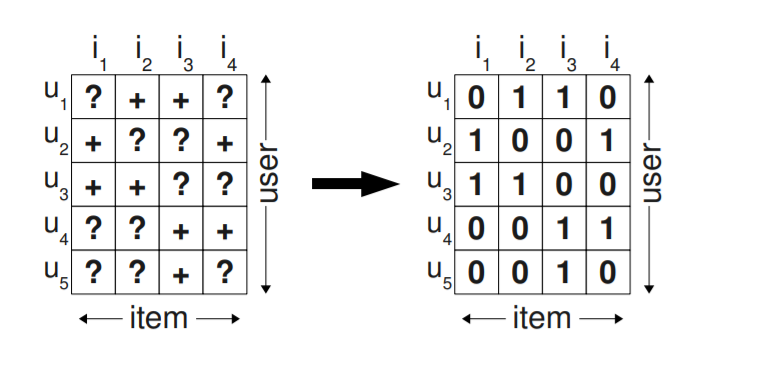
\includegraphics{images/BPR1.png}
    }
    
    \caption{
    \label{BPR1}
         }
    \end {center}
    \end {figure}
    Обычный подход заключается в том, чтобы предсказать
     персонализированную оценку для элемента, которая отражает 
     предпочтения пользователя для этого элемента. После этого 
     предметы будут ранжированы на основе этого балла. Здесь,
      как вы можете видеть на рисунке \ref{BPR1}, все существующие 
      взаимодействия между Пользователем и элементом помечаются как 
      положительный класс(1), а остальные взаимодействия помечаются
      как отрицательный класс(0).

      В подходе Байесовского
      персонализированного ранжирования, вместо взятия одного элемента, 
      будут рассматриваться пары элементов как обучающие данные.  Набор
         данных, который будет рассматриваться, сформулирован следующим
          образом 
          \begin{equation}
            (u,i,j) \in D_S
            \label{eq:1}
          \end{equation}
          
          \begin{figure}[ht]
            \begin{center}
            \scalebox{0.3}{
               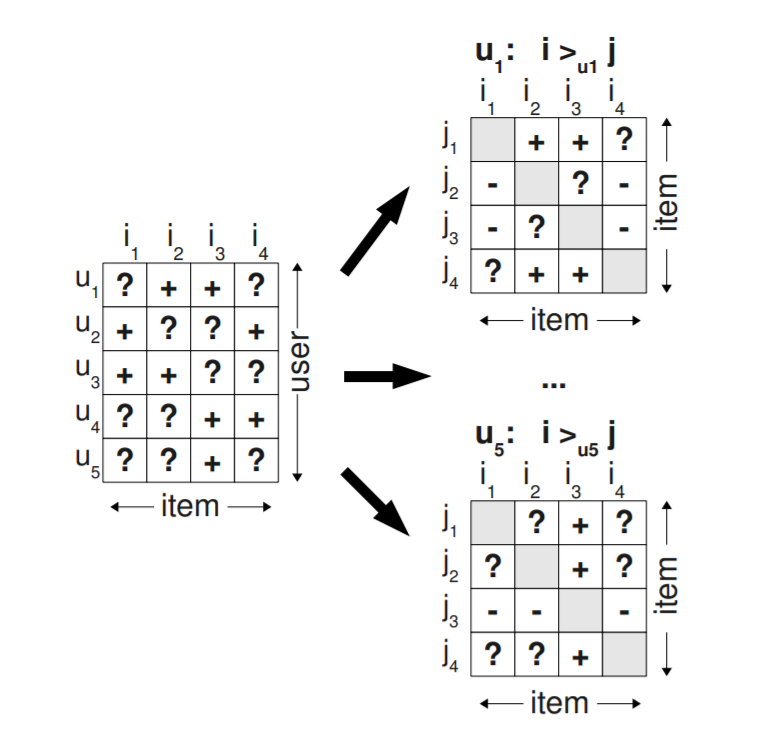
\includegraphics{images/BPR2.png}
            }
            
            \caption{
            \label{BPR2}
                 }
            \end {center}
            \end {figure}

            Здесь триплеты, сгенерированные для обучающих данных, представляют собой специфические для пользователя попарные предпочтения между парой элементов.
            

      \begin{equation}
        p(\Theta| >_u) \propto p(>_u| \Theta)p(\Theta)
        \label{eq:lik}
      \end{equation}

      Функция правдоподобия (\ref{eq:lik}), где ${>_u}$ -- это необходимые, 
      но латентные предпочтения структуры для пользователя $u$.

      Предполагая, что пользователи будут действовать независимо и порядок 
      каждой пары элементов ${(i, j)}$ для конкретного пользователя не зависит 
      от порядка каждой другой пары, мы можем сформулировать индивидуальную 
      вероятность того, что пользователь предпочитает элемент $i$ элементу $j$ 
      следующим образом:
      \begin{equation}
        p(i >_u j|\Theta) := \sigma(\hat x_{uij}(\Theta))
        \label{eq:ver}
      \end{equation}
    где $\sigma$ логистическая сигмоида: 
    \begin{equation}
        \sigma(x) := \frac{1}{1+e^{-x}}
        \label{eq:sigm}
      \end{equation}

${\hat x_{uij}(\Theta)}$ -- это в приведенном выше уравнении (\ref{eq:ver}) является 
вещественной значимой функцией, которая представляет собой отношение 
между пользователем $u$, элементом $i$ и элементом $j$ и обычно вычисляется 
с использованием модели матричного факторизации. Сигмовидная 
функция (\ref{eq:sigm}) дает индивидуальную вероятность, которая будет оптимизирована в 
ходе процесса.

${p(\Theta)}$ - это априорная вероятность, представляющая собой нормальное 
распределение с нулевым средним и дисперсионно-ковариационной матрицей.
\begin{equation}
    p(\Theta) \sim N(0, \Sigma_{\Theta})
    \label{eq:apr}
  \end{equation} 

  Следующее уравнение (\ref{eq:opt}) является окончательным критерием Байесовского
  персонализированного ранжирования, который должен быть оптимизирован
  \begin{equation}
    \sum_{(u,i,j)\in D_S} \ln \sigma(\hat x_{uij}) - \lambda_\Theta||\Theta||^2
    \label{eq:opt}
  \end{equation} 
  где $\lambda_\Theta$ -- специфические параметры регуляризации модели.

  \subsection{Реализация на языке программирования Python}
  Выберем порог оценки элемента, выше которого оценка считается положительной.
  Для дальнейшей работы представляем данные в виде разряженной таблицы, для более быстрой работы с большими таблицами.
  Разделяем исходные данные на тренировочную и тестовую выборки, 80\% данных на 
  тренировочную и 20\% на тестовую. На тренировочной выборке строим алгоритм рекомендаций байесовского
  персонализированного ранжирования.

  Далее реализуем метрики для проверки качества полученных рекомендаций.
  В качестве метрики для проверки точности рекомендаций используем precision (\ref{eq:prec}) (точность),
  а в качестве метрики сравнения исходного распределения и полученного, будем использовать
  дивергенцию Кульбака-Лейблера (\ref{eq:KL}). Для проверки будем брать
  30 лучших рекомндаций для пользователя.

  Калибровку рекомедаций будем производить двумя методами: первый (\ref{eq:Calibrated})
  основан на дивергенции Кульбака-Лейблера, а второй является 
  адаптацией метода Сент-Лагю \cite{bib5}.

Для сравнения с готовым решением будем использовать фреймворк SurPRISE \cite{sur} на языке программирования Python.
Из набора реализованных во фреймворке методов используем основанный на предположении о нормальном распределении NormalPredictor.
